\documentclass{beamer}
\usetheme{Szeged}
\usecolortheme{beaver}
\useoutertheme{infolines}

\usepackage{natbib}
\bibliographystyle{plain}

\usepackage{tikz}
\usetikzlibrary{bayesnet}

\author{Jacob Verdegaal \\Eli Drumm \\Bill Noble}
\title{Unsupervised Semantic Frame Induction}
\date{16 December, 2014}

\begin{document}

\begin{frame}
\maketitle
\end{frame}

\section{Semantic Frame Models}

\subsection{Model 0}
\begin{frame}
\begin{figure}
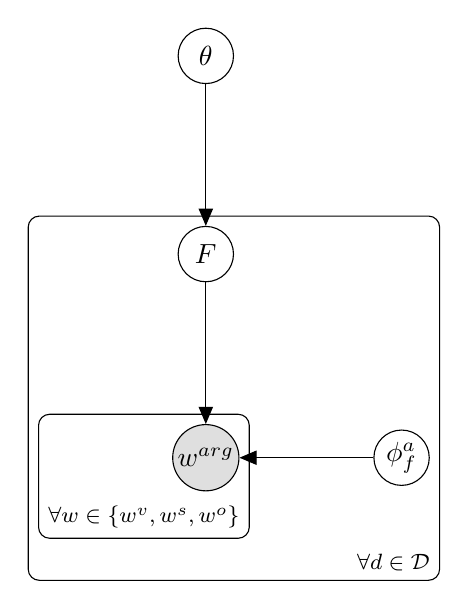
\begin{tikzpicture}[x=1.7cm,y=1.8cm]
    % Nodes
    \node[obs] (T) {$w^{arg}$} ; %
    \node[latent, above=of T] (F) {$F$} ; %
    \node[latent, above=of F] (theta) {$\theta$}; %
    \node[latent, right=of T] (phi) {$\phi^a_f$}; %
    \edge {theta} {F} ; %
    \edge {F} {T}
    \edge {phi} {T} ; %
    \plate {tuples} { (T) } {$\forall w \in \{w^v,w^s,w^o\}$}; %
    \plate {} { (tuples) (F) (phi)} {$\forall d \in \mathcal{D}$} ; %
\end{tikzpicture}
\end{figure}
\end{frame}

\subsection{Model 1}
\begin{frame}
\begin{figure}
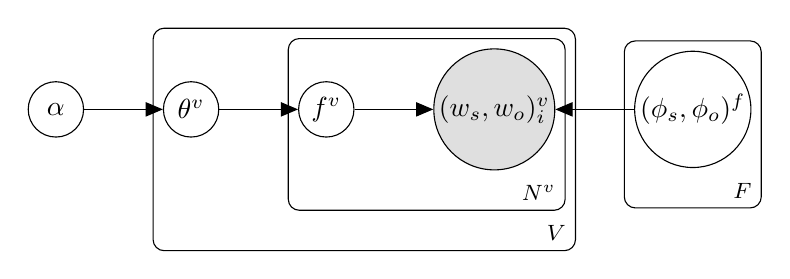
\begin{tikzpicture}[]
    \node[obs]                   (w)     {$(w_s,w_o)^v_i$}; %
    \node[latent, left=of w]     (f)     {$f^v$};
    \node[latent, left=of f]     (theta) {$\theta^v$};
    \node[latent, left=of theta] (alpha) {$\alpha$};
    \node[latent, right=of w]    (phi)   {$(\phi_s,\phi_o)^f$};
    \edge {alpha} {theta};
    \edge {theta} {f};
    \edge {f} {w};
    \edge {phi} {w};
    \plate {frames} {(phi)} {$F$};
    \plate {datapoints} {(f) (w)} {$N^v$};
    \plate {verbs} {(f) (w) (datapoints) (theta)} {$V$};
\end{tikzpicture}
\end{figure}


\end{frame}

\section{Results}

\section{References}
\begin{frame}[t,allowframebreaks]
\nocite{*}
\bibliography{refs.bib}
\end{frame}

\end{document}
